% vim: set spell spelllang=en tw=100 et sw=4 sts=4 :

\documentclass[20pt,a1paper,landscape]{tikzposter}

\usepackage{complexity}
\usepackage{wrapfig}
\usepackage{microtype}
\usepackage{gnuplot-lua-tikz}

\usepackage{lmodern}
\renewcommand*\familydefault{\sfdefault}
\usepackage[T1]{fontenc}

\title{Solving Hard Graph Problems in Parallel}
\author{Ciaran McCreesh and Patrick Prosser}
\institute{University of Glasgow, Glasgow, Scotland}
\titlegraphic{
\includegraphics[keepaspectratio=true,scale=2]{UoG_keyline.eps}}

\settitle{
    \begin{tikzpicture}
        \node (T) [inner sep=0pt] {\begin{minipage}{\linewidth}
                \color{titlefgcolor}
                {\bfseries \Huge \hspace{10mm}\@title \par}
                \vspace*{1em}
                {\Large {\bfseries \hspace{10mm}\@author}, \@institute}
        \end{minipage}};

        \node at (T.east) [anchor=center, inner sep=0pt, xshift=-8cm] {\@titlegraphic};
    \end{tikzpicture}
}

% University of Glasgow standard colours

\definecolor{uofgblue}{rgb}{0, 0.321569, 0.533333}
\colorlet{uofgblue20}{uofgblue!20!white}
\colorlet{uofgblue40}{uofgblue!40!white}
\colorlet{uofgblue60}{uofgblue!60!white}
\colorlet{uofgblue80}{uofgblue!80!white}

\definecolor{uofgstone}{rgb}{0.498039, 0.454902, 0.403922}
\colorlet{uofgstone40}{uofgstone!40!white}

\definecolor{uofgtdarkgreen}{rgb}{0.380392, 0.564706, 0.501961}
\definecolor{uofgtlightgreen}{rgb}{0.615686, 0.788235, 0.729412}
\definecolor{uofgtyellow}{rgb}{0.85098, 0.827451, 0.643137}
\definecolor{uofgtorange}{rgb}{0.784314, 0.694118, 0.545098}

\definecolorstyle{UofG}{
}{
    % Background Colors
    \colorlet{backgroundcolor}{uofgstone}
    \colorlet{framecolor}{black}
    % Title Colors
    \colorlet{titlefgcolor}{white}
    \colorlet{titlebgcolor}{uofgblue}
    % Block Colors
    \colorlet{blocktitlebgcolor}{white}
    \colorlet{blocktitlefgcolor}{uofgblue}
    \colorlet{blockbodybgcolor}{white}
    \colorlet{blockbodyfgcolor}{black}
    % Innerblock Colors
    \colorlet{innerblocktitlebgcolor}{uofgblue}
    \colorlet{innerblocktitlefgcolor}{black}
    \colorlet{innerblockbodybgcolor}{uofgstone}
    \colorlet{innerblockbodyfgcolor}{black}
    % Note colors
    \colorlet{notefgcolor}{black}
    \colorlet{notebgcolor}{uofgtlightgreen}
    \colorlet{noteframecolor}{red}
}

\usetheme{Autumn}
\usecolorstyle{UofG}

\tikzposterlatexaffectionproofoff

\useblockstyle[bodyverticalshift=-1cm, roundedcorners=1]{Default}

\renewcommand{\Huge}{\fontsize{61.92}{77}\selectfont}

% Styles for drawings

\tikzset{edge/.style={line width=3pt, color=uofgstone40}}
\tikzset{bedge/.style={line width=3pt}}
\tikzset{edgel1/.style={line width=3pt, color=uofgblue}}
\tikzset{edgel2/.style={line width=3pt, color=uofgblue40}}
\tikzset{edgel3/.style={line width=3pt, color=uofgtorange}}
\tikzset{edgel4/.style={line width=3pt, color=uofgtdarkgreen}}

% Colours for the graph lines

\colorlet{gp lt color 0}{uofgblue}
\colorlet{gp lt color 1}{uofgblue60}
\colorlet{gp lt color 2}{uofgblue20}
\colorlet{gp lt color 3}{uofgtorange}

\begin{document}
\maketitle

\block[bodyverticalshift=0cm, bodyinnersep=3mm]{}{\hspace{7mm}\emph{Exactly solving a hard graph problem
can take a long time. How can we exploit the parallelism offered by current multi-core processors to
speed things up, or to allow us to tackle larger or harder problems in the time we have?}}

\begin{columns}
\column{0.38}

\block{The Maximum Clique Problem}{
\begin{wrapfigure}[10]{r}{0.36\linewidth}
    \begin{center}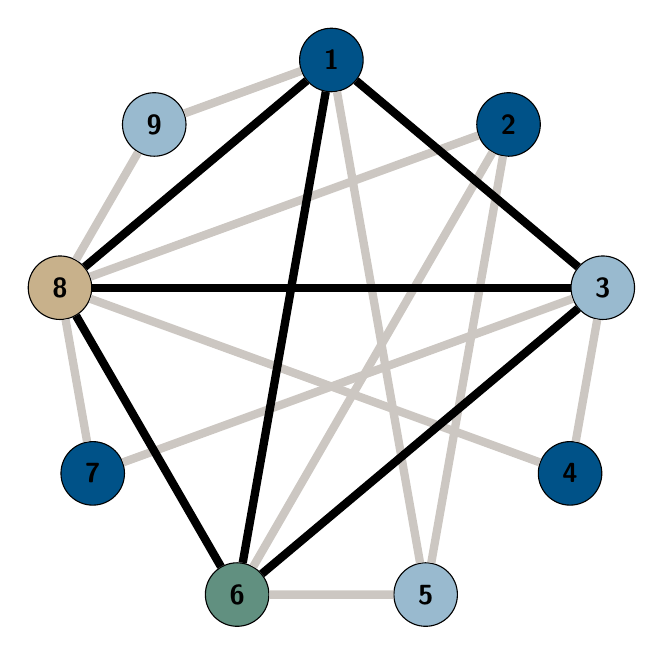
\begin{tikzpicture}[scale=1.75]%{{{
        \newcount \c
        \foreach \n in {1, ..., 9}{
            \c=\n
            \multiply\c by -40
            \advance\c by 130

            \ifthenelse{\n = 1 \OR \n = 2 \OR \n = 4 \OR \n = 7}{
                \node [draw, circle, fill=uofgblue, inner sep=5pt, font=\bfseries] (N\n) at (\the\c:2) {\n};
            }{
                \ifthenelse{\n = 3 \OR \n = 5 \OR \n = 4 \OR \n = 7 \OR \n = 9}{
                    \node [draw, circle, fill=uofgblue40, inner sep=5pt, font=\bfseries] (N\n) at (\the\c:2) {\n};
                }{
                    \ifthenelse{\n = 6}{
                        \node [draw, circle, fill=uofgtdarkgreen, inner sep=5pt, font=\bfseries] (N\n) at (\the\c:2) {\n};
                    }{
                        \node [draw, circle, fill=uofgtorange, inner sep=5pt, font=\bfseries] (N\n) at (\the\c:2) {\n};
                    }
                }
            }
        }

        \draw [edge] (N1) -- (N5); \draw [edge] (N1) -- (N9);
        \draw [edge] (N2) -- (N5); \draw [edge] (N2) -- (N6); \draw [edge] (N2) -- (N8);
        \draw [edge] (N3) -- (N4); \draw [edge] (N3) -- (N7);
        \draw [edge] (N4) -- (N8);
        \draw [edge] (N5) -- (N6);
        \draw [edge] (N7) -- (N8);
        \draw [edge] (N8) -- (N9);

        \draw [bedge] (N1) -- (N3);
        \draw [bedge] (N6) -- (N8);
        \draw [bedge] (N1) -- (N6);
        \draw [bedge] (N1) -- (N8);
        \draw [bedge] (N3) -- (N6);
        \draw [bedge] (N3) -- (N8);
    \end{tikzpicture}\end{center}
\end{wrapfigure}

A \textbf{clique} in a graph is a set of vertices, where every pair of vertices in the set are
adjacent. Finding a maximum clique is \NP-hard.

\bigskip

We can \textbf{grow candidate cliques} by recursively selecting a vertex for inclusion, and
rejecting non-adjacent vertices.  If we can colour a graph using $k$ colours, giving adjacent
vertices different colours, then the graph cannot contain a clique with more than $k$ vertices. This
gives a \textbf{branch and bound algorithm}: a greedy colouring of the undecided vertices determines
whether we might be able to beat the best clique found so far.
}

\block{Parallel Tree-Search}{
    We can see the recursive calls made as forming a tree. Triangles represent large subtrees;
    the~$\star$ marks the best solution. Light blue subtrees are those which could be eliminated by
    the bound, if the best solution has already been found: we call these \textbf{eliminable}. The
    leftmost eliminable tree below will be explored in a sequential run; the others will not.

    \begin{center}\begin{tikzpicture}[scale=1.75]
        \coordinate (R);

        \coordinate (N) at (R);

        \coordinate (N1) at ($(N) + (-6, -0.75)$);
        \coordinate (N2) at ($(N) + (-2, -0.75)$);
        \coordinate (N3) at ($(N) + ( 2, -0.75)$);
        \coordinate (N4) at ($(N) + ( 6, -0.75)$);

        \foreach \na in {1, ..., 4}{
            \coordinate (N\na 1) at ($(N\na) + (-1.25, -1)$);
            \coordinate (N\na 2) at ($(N\na) + ( 0,    -1)$);
            \coordinate (N\na 3) at ($(N\na) + ( 1.25, -1)$);

            \foreach \nb in {1, ..., 3}{
                \coordinate (N\na\nb t1) at ($(N\na\nb) + (-0.5, -1)$);
                \coordinate (N\na\nb t2) at ($(N\na\nb) + ( 0.5, -1)$);
            }
        }

        \foreach \na in {1, ..., 4}{
            \draw (N) -- (N\na);
            \foreach \nb in {1, ..., 3}{
                \draw (N\na) -- (N\na\nb);
            }
        }

        \tikzstyle{t} = [draw, fill, fill=uofgblue, rounded corners=3mm];
        \tikzstyle{u} = [draw, fill, fill=uofgblue20, rounded corners=3mm];
        \foreach \na in {1, ..., 4}{
            \foreach \nb in {1, ..., 3}{
                \ifthenelse{\na\nb = 13 \OR \na\nb = 32 \OR \na\nb = 33 \OR \na = 4}{
                    \draw [u] (N\na\nb) -- (N\na\nb t1) -- (N\na\nb t2) -- cycle;
                }{
                    \draw [t] (N\na\nb) -- (N\na\nb t1) -- (N\na\nb t2) -- cycle;
                }
            }
        }

        \tikzstyle{c} = [draw, circle, fill, fill=uofgblue];
        \tikzstyle{e} = [draw, circle, fill, fill=uofgblue20];
        \node [c] at (N) { };

        \foreach \na in {1, ..., 4}{
            \ifthenelse{\na = 4}{
                \node [e] at (N\na) { };
            }{
                \node [c] at (N\na) { };
            }

            \foreach \nb in {1, ..., 3}{
                \ifthenelse{\na\nb = 13 \OR \na\nb = 32 \OR \na\nb = 33 \OR \na = 4}{
                    \node [e] at (N\na\nb) { };
                }{
                    \node [c] at (N\na\nb) { };
                }
            }
        }

        \tikzstyle{p} = [draw, rounded corners, dashed, color=uofgtorange, line width=3pt];
        \foreach \na in {1, ..., 4}{
            \foreach \nb in {1, ..., 3}{
                \draw [p] ($(N\na\nb) + (-0.55, 0.51)$) -- ($(N\na\nb) + (0.55, 0.51)$) --
                    ($(N\na\nb) + (0.55, -1.5)$) -- ($(N\na\nb) + (-0.55, -1.5)$) -- cycle;
                }
        }

        \node [c] at (N21t1) { };
        \node at (N21t1) { $\star$ };
    \end{tikzpicture}\end{center}

    We can explore subtrees in parallel, by allocating subtrees to workers. But the problem is
    \textbf{irregular}: some subproblems may be orders of magnitude larger than others.  We solve
    this by creating a queue with \textbf{many more subproblems} than we have workers, like in
    Embarrasingly Parallel Search.

    \bigskip

    This parallelism is \textbf{speculative}. If one worker gets lucky and finds $\star$ quickly, we
    could do less overall work, and get a \textbf{superlinear speedup} by avoiding some of the
    eliminable subtrees that would have been explored sequentially. On the other hand, our extra
    workers could contribute nothing at all, by exploring more eliminable subtrees. We \emph{can}
    guarantee that \textbf{we will never introduce a slowdown}, by communicating bounds and
    preserving sequential ordering.
}

\column{0.38}

\block{Balance versus Search Order}{
    \begin{center}
    \begin{tikzpicture}
        \input{gen-graph-speedup}
    \end{tikzpicture}
    \end{center}

    Splitting further down the tree improves balance, but often gives worse results. This is partly
    due to overheads, but is also because \textbf{heuristics are weakest at the top of search}, and
    splitting high introduces diversity.  We can get the best of both worlds, \emph{and} reduce
    the total number of queue operations, by splitting high first for diversity, and then
    resplitting later for balance.
}

\block{Flexibility and Related Problems}{
    Dedicated clique algorithms are surprisingly flexible. Sophisticated MIP models cannot
    be adapted for the \textbf{maximum labelled clique} problem (left), but clique algorithms can
    be, and are very effective in practice. We can also incorporate symmetry removal, for the
    \textbf{maximum balanced induced biclique} problem (center), and dominance removal, for the
    \textbf{maximum $k$-clique problem} (right).

    \vspace{0.5cm}
    \begin{center}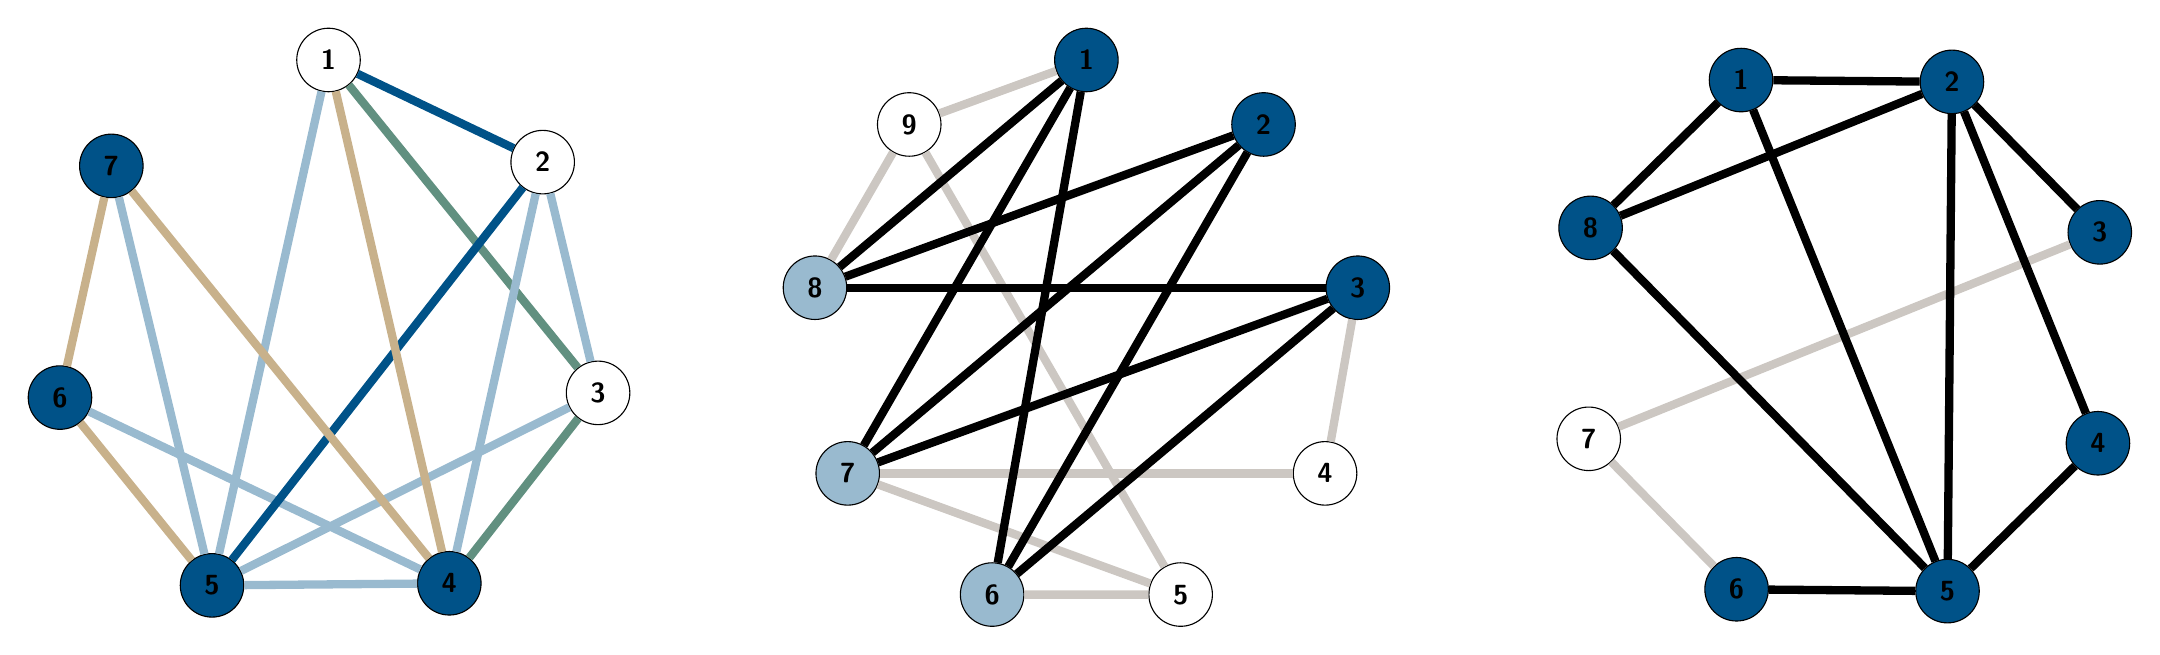
\begin{tikzpicture}[scale=1.75]
        \newcount \myc

        \begin{scope}
            \foreach \n in {1, ..., 7}{
                \myc=\n \advance\myc by -1 \multiply\myc by -360 \divide\myc by 7 \advance\myc by 90
                \ifthenelse{\n=4 \OR \n=5 \OR \n=6 \OR \n=7}{
                    \node [fill=uofgblue, draw, circle, inner sep=5pt, font=\bfseries] (N\n) at (\the\myc:2) {\n};
                }{
                    \node [draw, circle, inner sep=5pt, font=\bfseries] (N\n) at (\the\myc:2) {\n};
                }
            }

            \draw [edgel4] (N3) -- (N4);
            \draw [edgel4] (N1) -- (N3);
            \draw [edgel2] (N1) -- (N5);
            \draw [edgel2] (N2) -- (N3);
            \draw [edgel2] (N2) -- (N4);
            \draw [edgel2] (N3) -- (N5);
            \draw [edgel2] (N4) -- (N5);
            \draw [edgel2] (N4) -- (N6);
            \draw [edgel2] (N5) -- (N7);
            \draw [edgel1] (N1) -- (N2);
            \draw [edgel1] (N2) -- (N5);
            \draw [edgel3] (N4) -- (N7);
            \draw [edgel3] (N5) -- (N6);
            \draw [edgel3] (N6) -- (N7);
            \draw [edgel3] (N1) -- (N4);
        \end{scope}

        \begin{scope}[xshift=5.5cm]
            \foreach \n in {1, ..., 9}{
                \myc=\n
                \multiply\myc by -40
                \advance\myc by 130
                \ifthenelse{\n=1 \OR \n=2 \OR \n = 3}{
                    \node [fill=uofgblue, draw, circle, inner sep=5pt, font=\bfseries] (N\n) at (\the\myc:2) {\n};
                }{}

                \ifthenelse{\n=6 \OR \n=7 \OR \n = 8}{
                    \node [fill=uofgblue40, draw, circle, inner sep=5pt, font=\bfseries] (N\n) at (\the\myc:2) {\n};
                }{}

                \ifthenelse{\n=4 \OR \n=5 \OR \n = 9}{
                    \node [draw, circle, inner sep=5pt, font=\bfseries] (N\n) at (\the\myc:2) {\n};
                }{}
            }

            \draw [edge] (N1) -- (N9);
            \draw [edge] (N3) -- (N4);
            \draw [edge] (N4) -- (N7);
            \draw [edge] (N5) -- (N6);
            \draw [edge] (N5) -- (N7);
            \draw [edge] (N8) -- (N9);
            \draw [edge] (N5) -- (N9);

            \draw [bedge] (N1) -- (N6);
            \draw [bedge] (N1) -- (N7);
            \draw [bedge] (N1) -- (N8);
            \draw [bedge] (N2) -- (N8);
            \draw [bedge] (N2) -- (N7);
            \draw [bedge] (N2) -- (N6);
            \draw [bedge] (N3) -- (N8);
            \draw [bedge] (N3) -- (N7);
            \draw [bedge] (N3) -- (N6);
        \end{scope}

        \begin{scope}[xshift=11cm]
            \foreach \n in {1, ..., 8}{
                \myc=\n \advance\myc by -1 \multiply\myc by -360 \divide\myc by 8 \advance\myc by 90 \advance\myc by 22.5
                \ifthenelse{\n = 1 \OR \n = 2 \OR \n = 3 \OR \n = 4 \OR \n = 5 \OR \n = 6 \OR \n = 8}{
                    \node [fill=uofgblue, draw, circle, inner sep=5pt, font=\bfseries] (N\n) at (\the\myc:2) {\n};
                }{
                    \node [draw, circle, inner sep=5pt, font=\bfseries] (N\n) at (\the\myc:2) {\n};
                }
            }

            \draw [edge] (N3) -- (N7);
            \draw [edge] (N6) -- (N7);

            \draw [bedge] (N1) -- (N2);
            \draw [bedge] (N1) -- (N5);
            \draw [bedge] (N1) -- (N8);
            \draw [bedge] (N2) -- (N5);
            \draw [bedge] (N2) -- (N8);
            \draw [bedge] (N5) -- (N8);
            \draw [bedge] (N2) -- (N3);
            \draw [bedge] (N2) -- (N4);
            \draw [bedge] (N4) -- (N5);
            \draw [bedge] (N5) -- (N6);
        \end{scope}
    \end{tikzpicture}\end{center}
}

\column{0.24}
\block{Future Work}{
How about other problems, such as subgraph isomorphism, maximum common subgraph,
or graph colouring?

\bigskip

SAT solvers do not seem to parallelise well. But we can translate SAT and MaxSAT into
clique problems. Given enough processors, can this beat using a dedicated SAT solver?

\bigskip

Can these techniques scale to clusters of multi-core systems, by combining message passing and
threads?

\bigskip

In practice, splitting a problem up into linearly more pieces than there are cores
usually works reasonably well. But does this work in theory?

\bigskip

How do symmetries interact with parallel search algorithms?
}

\def\bysame{\leavevmode\hbox to3em{\hrulefill}\thinspace}

\block{References}{
    \small
Ciaran McCreesh, Patrick Prosser: Multi-Threading a State-of-the-Art Maximum Clique Algorithm.
Algorithms 6(4): 618-635 (2013)

\bigskip

\bysame: An Exact Branch and Bound Algorithm with Symmetry Breaking for the
Maximum Balanced Induced Biclique Problem. CPAIOR 2014: 226-234

\bigskip

\bysame: Reducing the Branching in a Branch and Bound Algorithm for the
Maximum Clique Problem. CP 2014: 549-563

\bigskip

\bysame: The Shape of the Search Tree for the Maximum Clique Problem, and
the Implications for Parallel Branch and Bound. CoRR abs/1401.5921 (2014)

\bigskip

\bysame: A Parallel Branch and Bound Algorithm for the Maximum Labelled Clique Problem. CoRR
abs/1407.7061 (2014)

\bigskip

\bysame: Finding Maximum $k$-Cliques Faster using Lazy Global Domination. CoRR
abs/1408.6485 (2014)

}

\block[bodyverticalshift=0cm]{}{
    \texttt{c.mccreesh.1@research.gla.ac.uk}

    \smallskip
    \small
    This work was supported by the Engineering and Physical Sciences Research Council [grant number
    EP/K503058/1]
}

\end{columns}

\end{document}

